\RequirePackage{lineno}
\documentclass[preprint,nofootinbib,showpacs,prl,superscriptaddress,secnumarabic,amssymb,nobibnotes,aps,floatfix]{revtex4}
\usepackage{graphicx}
\usepackage{hyperref}
\usepackage{amsmath}
\usepackage{dcolumn}% Align table columns on decimal point
\usepackage{bm}% bold math
%
\def\Dirac#1{#1\hskip-5pt/}
%
\newcommand*\patchAmsMathEnvironmentForLineno[1]{%
\expandafter\let\csname old#1\expandafter\endcsname\csname #1\endcsname
\expandafter\let\csname oldend#1\expandafter\endcsname\csname end#1\endcsname
\renewenvironment{#1}%
{\linenomath\csname old#1\endcsname}%
{\csname oldend#1\endcsname\endlinenomath}}%
\newcommand*\patchBothAmsMathEnvironmentsForLineno[1]{%
\patchAmsMathEnvironmentForLineno{#1}%
\patchAmsMathEnvironmentForLineno{#1*}}%
\AtBeginDocument{%
\patchBothAmsMathEnvironmentsForLineno{equation}%
\patchBothAmsMathEnvironmentsForLineno{align}%
\patchBothAmsMathEnvironmentsForLineno{flalign}%
\patchBothAmsMathEnvironmentsForLineno{alignat}%
\patchBothAmsMathEnvironmentsForLineno{gather}%
\patchBothAmsMathEnvironmentsForLineno{multline}%
}


%
\begin{document}
\linenumbers

\title{First Exclusive Measurement of Deep Virtual Compton Scattering off $^4$He: Toward the 3D tomography of nuclei}

\newcommand*{\ANL}{Argonne National Laboratory, Argonne, Illinois 60439}
\newcommand*{\ANLindex}{1}
\affiliation{\ANL}
\newcommand*{\ORSAY}{Institut de Physique Nucl\'eaire, CNRS/IN2P3 and Universit\'e Paris Sud, Orsay, France}
\newcommand*{\ORSAYindex}{2}
\affiliation{\ORSAY}
\newcommand*{\JLAB}{Thomas Jefferson National Accelerator Facility, Newport News, Virginia 23606}
\newcommand*{\JLABindex}{3}
\affiliation{\JLAB}
 
\newcommand*{\NOWJLAB}{Thomas Jefferson National Accelerator Facility, Newport News, Virginia 23606}
\newcommand*{\NOWODU}{Old Dominion University, Norfolk, Virginia 23529}
 %%%%%%%%%%%%%%% END OF Latex Macros for institute addresses  %%%%%%%%%%%%%%%%%%%%%%%%% 

\author {M.~Hattawy}
\affiliation{\ANL}
\affiliation{\ORSAY}
\author {R.~Dupr\'{e}} 
\affiliation{\ANL}
\affiliation{\ORSAY}
\author {N.A.~Baltzell} 
\affiliation{\ANL}
\affiliation{\JLAB}
\author {K.~Hafidi} 
\email[corresponding author: ]{kawtar@anl.gov}
\affiliation{\ANL}


\collaboration{The CLAS Collaboration}
\noaffiliation

%
\date{\today}
\begin{abstract}
We report the first fully exclusive measurement of deeply virtual Compton 
scattering (DVCS) off a nucleus for $A>1$. The experiment used the 6 GeV 
electron beam from Jefferson Lab projected onto a $^4$He target in the center 
of the CEBAF Large Acceptance Spectrometer (CLAS). An additional radial time 
projection chamber (RTPC) was used to detect the recoiling $^4$He nuclei and 
ensure the exclusivity of the process. We measured beam spin asymmetries 
significantly larger than that observed on proton targets and extracted,
in a completely model independent way, the chiral even generalized parton 
distribution (GPD) of the $^4$He nucleus. This pioneering measurement 
leads the way toward the 3D imaging of the partonic structure of nuclei.
\end{abstract}
\pacs{Valid PACS appear here}

\maketitle 

A wealth of information on quantum chromodynamics (QCD) lies in the 
internal structure of hadrons. In the recent past, development of the 
generalized parton distributions (GPDs) framework has offered the possibility
to obtain new information about the momentum and spatial degrees of 
freedom of the quark and gluons inside hadrons 
\cite{Mueller:1998fv,Ji:1996ek,Ji:1996nm,Radyushkin:1996nd,Radyushkin:1997ki}.
In impact parameter space, the GPDs are indeed interpreted as a tomography of the 
transverse plane for partons carrying a certain longitudinal momentum 
\cite{Burkardt:2000za,Diehl:2002he,Belitsky:2002ep,Burkardt:2005hp}. 

The main access to GPDs is through the measurement of deep virtual Compton 
scattering (DVCS), i.e. the hard exclusive electroproduction of a real photon. 
While other processes are known to be sensitive to GPDs, the measurement of
DVCS is considered the cleanest probe and has been the focus of a worldwide effort 
\cite{Stepanyan:2001sm,Airapetian,Chekanov:2003ya,Aktas:2005ty,Chen:2006na,Munoz 
Camacho:2006hx,Girod:2007aa,Mazouz:2007aa,Gavalian:2009,Seder:2015,Pisano:2015,Jo:2015ema} 
[Should we cite less publications on the topic or a review?]
involving several accelerator facilities such as Jefferson Lab (JLab), HERA and  
CERN. The vast majority of these measurements focused on the study of 
proton structure and allowed extraction of the tomography of the nucleon (for details on the formalism, see 
\cite{Goeke:2001tz,Diehl:2003ny,Ji:2004gf,Belitsky:2005qn,Boffi:2007yc,Guidal:2013rya}).
This framework is also applicable to nuclei, giving access to completely new 
information about nuclear structure in terms of quarks and 
gluons \cite{Dupre:2015jha}.
Study of the 3D structure of nuclei appears to be especially important
in light of the large nuclear effects observed in nuclear parton distribution 
functions \cite{Geesaman:1995yd,Norton:2003cb,Hen:2016kwk}.

\begin{figure}[tb]
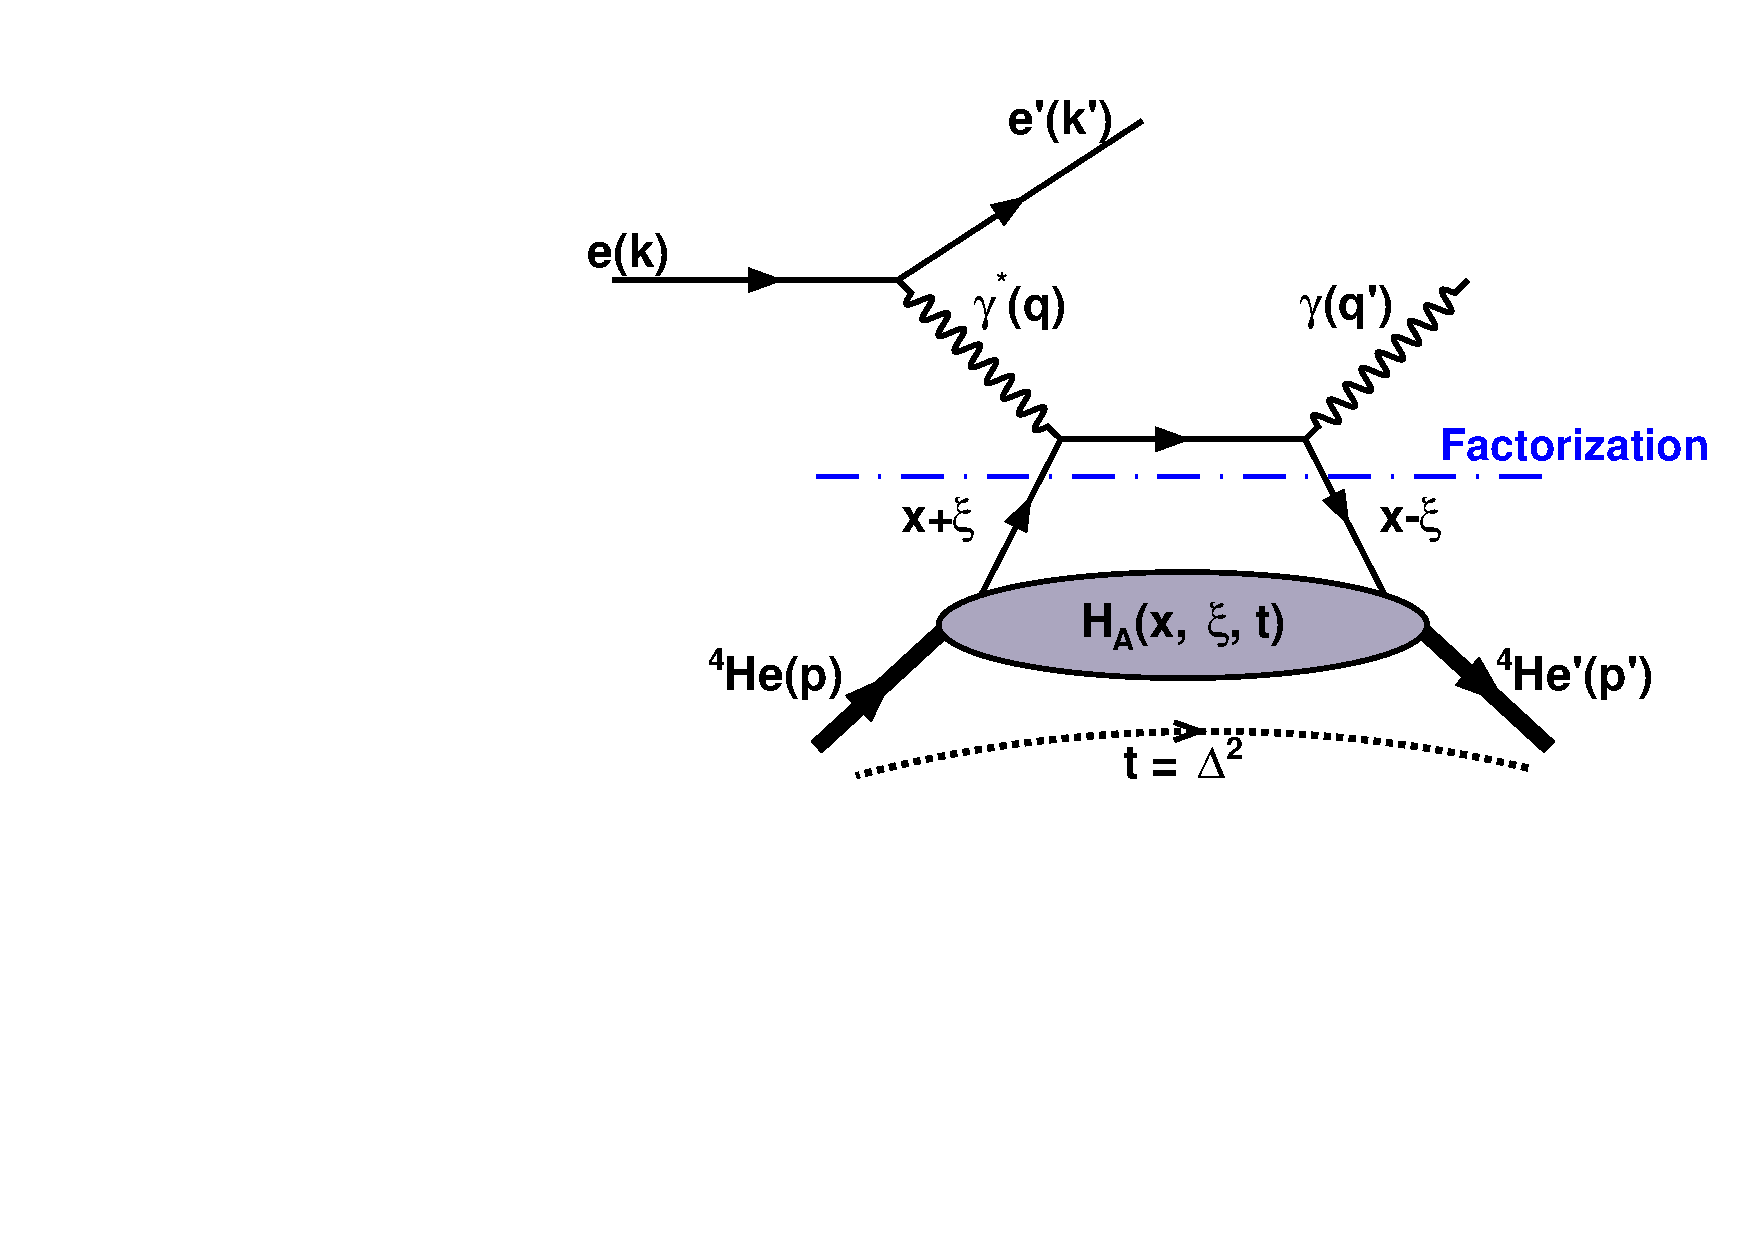
\includegraphics[width=6.5cm]{figs/DVCS_diagram.pdf}
\caption{Representation of the leading-order, twist-2, handbag diagram of the 
DVCS process off $^4$He.}
\label{fig:diags}
\end{figure}

The coherent nuclear DVCS channel is experimentally difficult due to  
its small cross section and the necessity to ensure the target remains 
intact while emitting a hard photon ($eA \rightarrow e' A' \gamma$). Figure 
\ref{fig:diags} illustrates the hand bag diagram for coherent DVCS on 
$^4$He. Similar to the proton case, at large virtual photon's 4-momentum square 
$Q^2=-(k-k')^{2}$ and small squared momentum transfer $t=(p-p')^{2}$,
the DVCS handbag diagram can be factorized into two parts 
\cite{Freund_Collins,Ji_Osborne}. The hard part includes the photon-quark 
interaction and is calculable with perturbative QED.  The non-perturbative 
part is parametrized in terms of GPDs, which embed the partonic structure of 
the hadron. The GPDs depend on the three variables $x$, $\xi$ and $t$, which are 
indicated in Figure \ref{fig:diags} for the DVCS process. In DVCS, $\xi$ can 
be related to the Bjorken variable $x_{B}$: $\xi\approx {{x_B}\over{2-x_B}}$, 
where $x_B=\frac{Q^2}{2M\nu}$ with $M$ the proton mass and 
$\nu=E_e-E_{e^\prime}$. One can access $t$ as the squared momentum 
transferred to the target, however $x$ cannot be experimentally 
accessed in a DVCS reaction. Hence, we measure only complex Compton Form 
Factors (CFF) \cite{Guidal:2013rya} defined as:
\begin{align}
\begin{split}
\Re e(&\mathcal{H}_{A}) = \\
    &\mathcal{P} 
\int_{0}^{1}dx[H_A(x,\xi,t)-H_A(-x,\xi,t)] \, C^{+}(x,\xi), 
\end{split} \\
\Im m(&\mathcal{H}_{A}) = H_A(\xi,\xi,t)-H_A(-\xi,\xi,t),
\end{align}
with $H_A$ the GPD, $\mathcal{P}$ 
the Cauchy principal value integral, and $C^{+}(x,\xi)$ a coefficient function 
($=  \frac{1}{x-\xi} + \frac{1}{x+\xi}$).

The main challenge in studying nuclear DVCS is ensuring the exclusivity of 
the reaction. Until now, the only available data set of nuclear DVCS
was from the HERMES experiment \cite{Ellinghaus:2002zw}, where exclusivity was 
based only on kinematic cuts on the measured scattered electron and real photon. 
That measurement was performed on a large set of nuclei ($^4$He, N, Ne, Kr and 
Xe), but the mixing of the coherent and incoherent processes could affect the
measurement significantly \cite{Guzey:2003jh}. In this regard, direct 
detection of the low-energy 
recoil nucleus is the best way to guarantee the nucleus remains intact and that 
the reaction did not occur on a bound nucleon. The 
CEBAF Large Acceptance 
Spectrometer (CLAS) in Hall-B at JLab is already optimized for 
DVCS measurements 
\cite{Girod:2007aa,Gavalian:2009,Seder:2015,Pisano:2015,Jo:2015ema}, 
so we built a dedicated radial time projection chamber (RTPC) for the detection of 
the recoiling low energy nuclei in order to complete this experimental setting.  
The $^4$He nucleus is an ideal experimental target in this regard, as it is 
light enough to be detected in such a setting, while it
is subject to significant nuclear effects \cite{JSeely} and has rather high 
density.  A helium target leads to another important advantage, as the number of GPDs 
defined for a hadron depends on its spin. The structure of a spin zero nucleus, such as 
$^4$He, is parametrized by only one chiral even GPD ($H_{A}(x,\xi,t)$) at 
leading twist, while 4 GPDs arise in the nucleon case. This significantly
simplifies the interpretation of the data and allows a model independent
extraction of the $^4$He CFF ($\mathcal{H}_{A}$) presented at the
end of this letter. 

%experimental setup

The experiment E08-024 took place in Hall-B at JLab
in 2009 using the nearly 100\% duty factor, longitudinally 
polarized electron beam (83$\%$ polarization) at its full energy of 6.064 
GeV. The data were collected over three months using a 6 atm gaseous $^4$He 
target placed in the center of CLAS. For DVCS experiments, the CLAS baseline 
design \cite{Mecking:2003zu} is supplemented with an inner calorimeter (IC) and 
a solenoid. The IC extends the photon detection acceptance of CLAS, which was 
originally from 15$^{\circ}$ to 45$^{\circ}$, to polar angles as low as 
4$^{\circ}$. At these small angles the low-energy M\o{}ller electrons produced 
in the target form a very high rate background that is
suppressed by a 5 Tesla solenoid placed around the target. 

Because the coherent DVCS cross section is peaked at low $-t$, the recoil 
$^4$He nuclei produced in DVCS have a low average momentum around 300 
MeV/c. CLAS cannot detect such low energy $\alpha$ particles, 
so in order to ensure the exclusivity of the measurement, we built a small and 
light RTPC to complement CLAS. Figure~\ref{fig:RTPC} presents the design of 
this RTPC and the $^4$He gaseous target in its center. The detector was 
calibrated specifically for the detection of
$^4$He nuclei based on elastic scattering with a 1.2~GeV electron beam.


\begin{figure}[tb]
\vspace{-1.1cm}
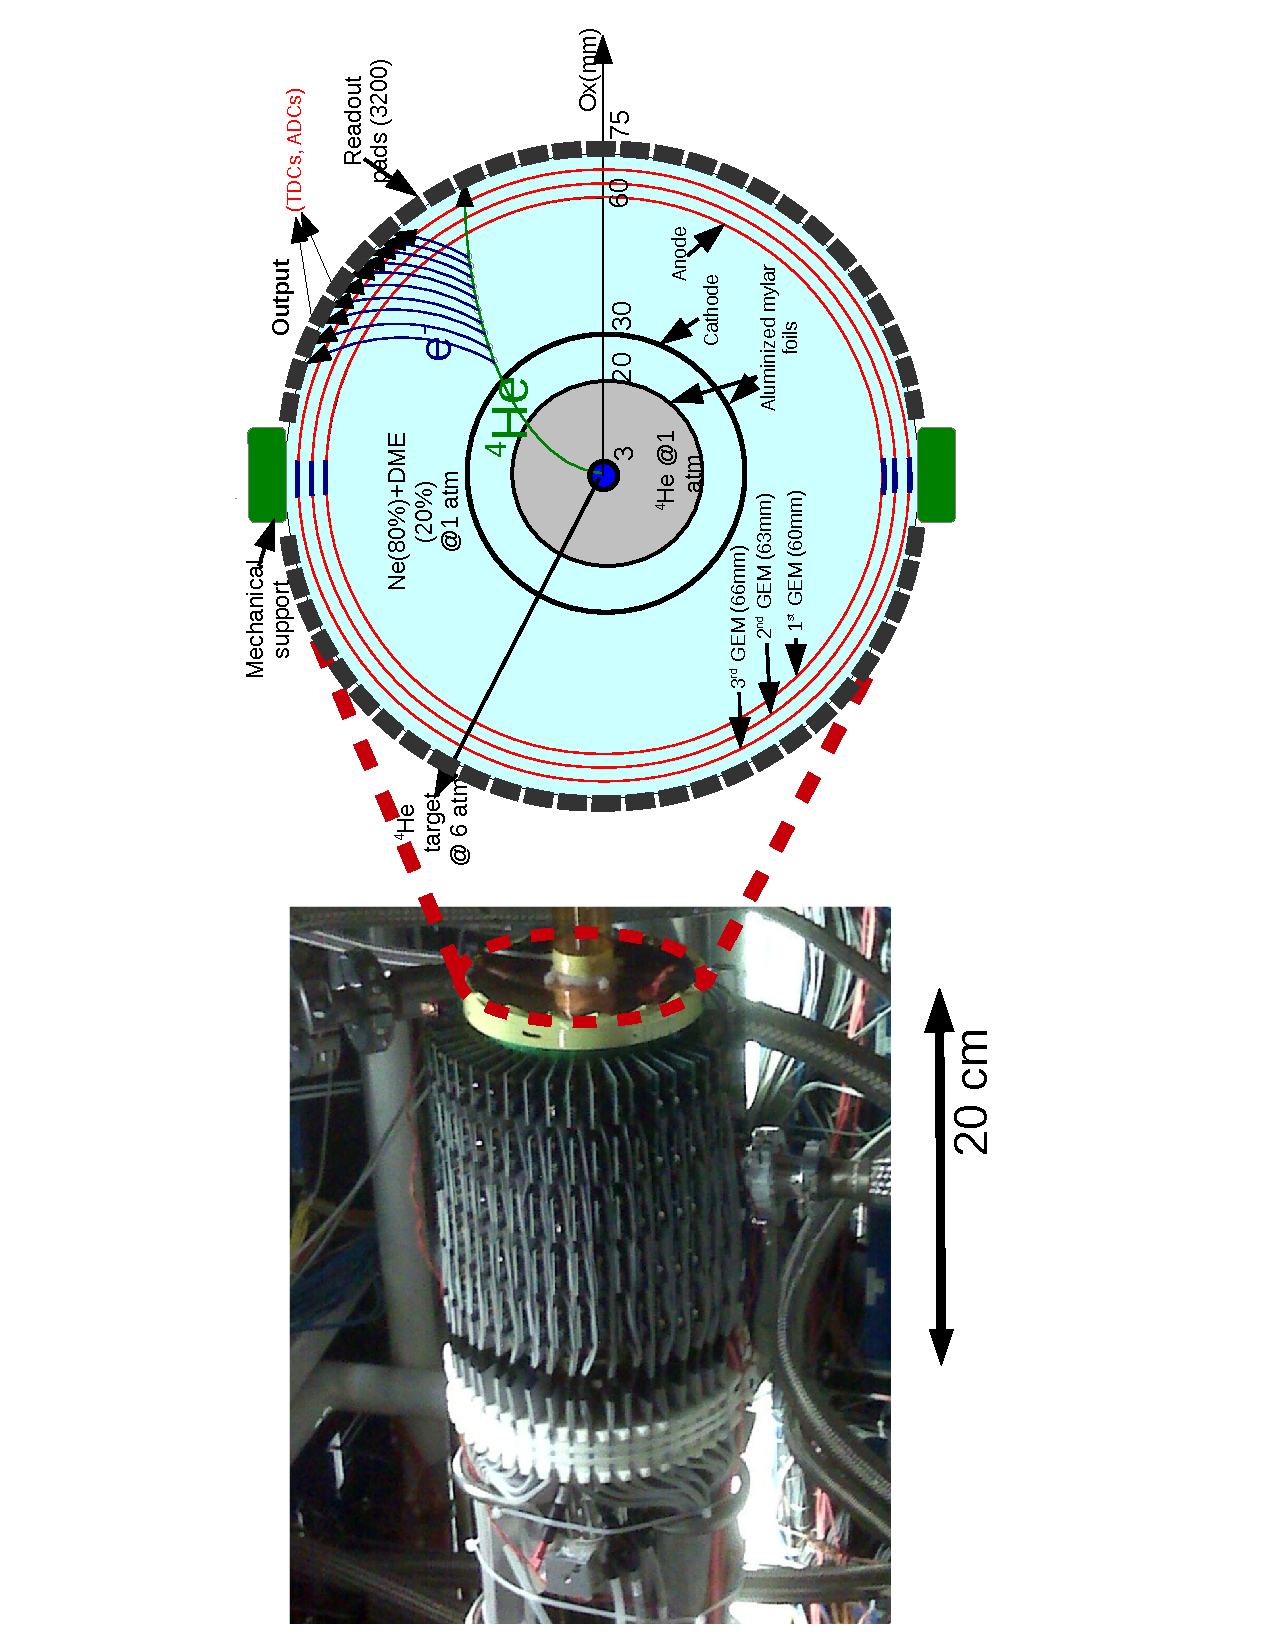
\includegraphics[width=7.0cm,angle=-90]{figs/RTPC.pdf}
\vspace{-1.1cm}
\caption{Left: A picture of the E08-024 RTPC before insertion into the 
   solenoid. Right: A cross section of the E08-024 RTPC perpendicular to the 
   beam direction. An illustration of a $^4$He track originating from the 
   pressurized straw target is shown along with the electrons produced in the 
   drift region.}
\label{fig:RTPC}
\end{figure}

%DVCS selection
To identify coherent DVCS events, we first select events where one 
electron, one $^4$He, and at least one photon are detected in the final state. 
Electrons are identified by using fiducial cuts and requiring appropriate
signals in all the sub-detectors of the baseline CLAS (drift chambers, 
Cherenkov counters, electromagnetic calorimeter, and time of flight 
scintillators). The $^4$He tracks are identified with fiducial, 
timing and track quality cuts in the RTPC detector. In addition,
we apply a vertex matching cut to ensure the electron and helium
nucleus originate from the same position. The photons are detected in either
the IC or the CLAS electromagnetic calorimeter.  Note that even though the 
DVCS reaction has only one real photon in the final state, 
events with more than one good photon are not discarded at this stage. This is 
motivated by the fact that, while soft photons are likely to be produced in random 
coincidence, they cannot be mistaken for the large energy DVCS photons ($>2$ GeV).
The most energetic photon is always considered as the DVCS photon candidate.

The main background in the measurement of DVCS is coherent $\pi^{0}$ 
production. Therefore, we remove events where a $\pi^{0}$ can be identified by 
invariant mass reconstruction of two photons.  To ensure the interaction 
occurs at the partonic level and the DVCS handbag diagram is dominant, we 
select events with $Q^{2}>1~[GeV^{2}/c^{2}]$. The exclusivity of the events is 
obtained by applying a set of cuts on the following kinematic variables: the 
co-planarity angle ($\Delta \phi$), the missing energy, the missing mass 
squared, the missing transverse momentum, the missing mass squared of the 
$e'^4He'$ system, and the angle ($\theta$) between the measured photon and the 
missing momentum of the $e'^4He'$ system. The most relevant of these cuts are 
presented in Figure~\ref{fig:kin-cuts}, which shows 3$\sigma$ cuts except for the 
missing energy (which appears to be too large and for which we reduced the cut 
window to [-0.45,0.5] GeV). After these requirements, we have about 3200 events 
left, and Figure \ref{fig:kin-coverage} presents their
kinematic distributions in ($Q^{2}$,$x_{B}$) and ($Q^{2}$,$-t$).

\begin{figure}[tb]
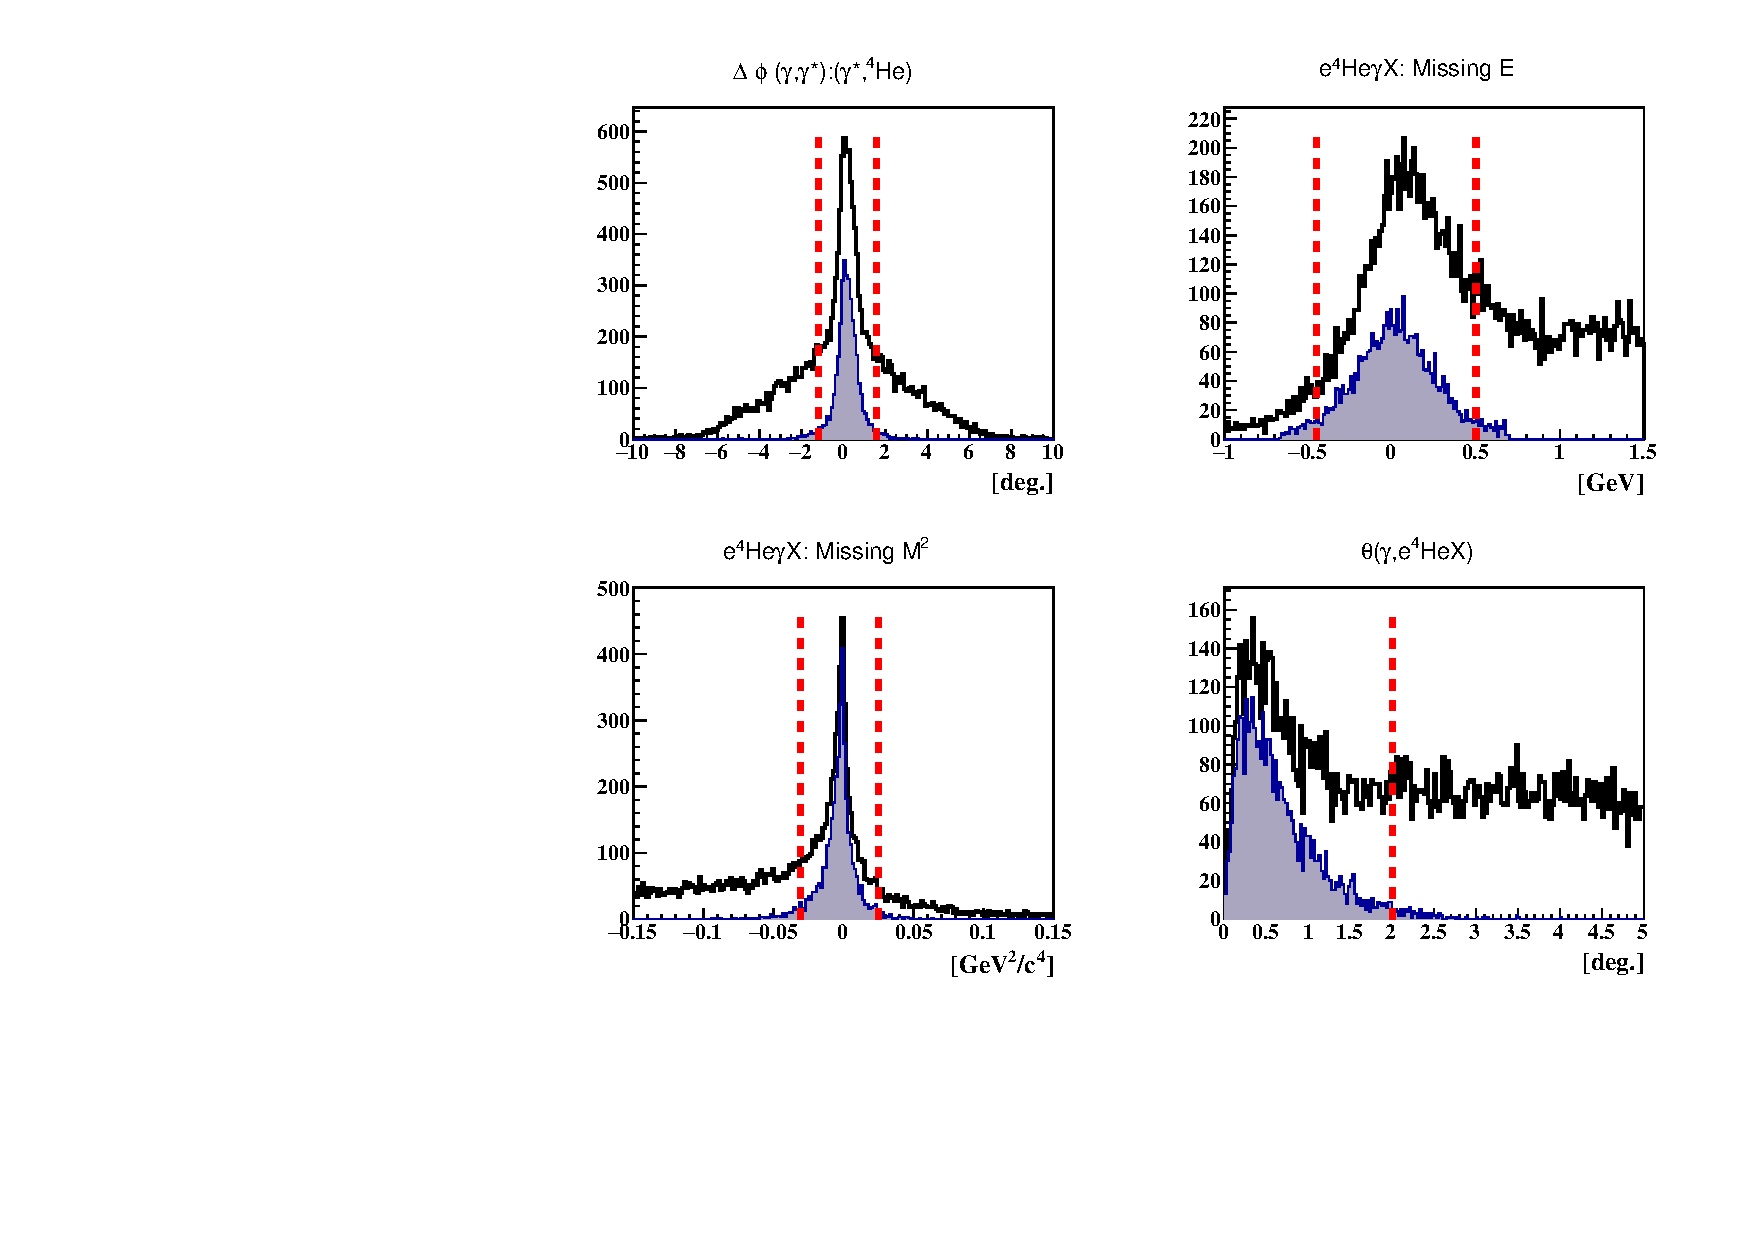
\includegraphics[width=8.9cm]{figs/coh_exc_cuts.pdf}
\caption{Four of the six coherent DVCS exclusivity cuts. The black 
distributions represent the coherent DVCS events candidate. The shaded 
distributions represent the events which passed all the exclusivity cuts except 
the quantity plotted. The vertical red lines represent the applied exclusivity 
cuts. The distributions from left to right and from top to bottoms are: $\Delta 
\phi$, missing energy, missing mass squared and the cone angle ($\theta$) 
between the measured and the calculated photons.}
\label{fig:kin-cuts}
\end{figure}
 

\begin{figure}[tb]
\hspace{-0.45cm}
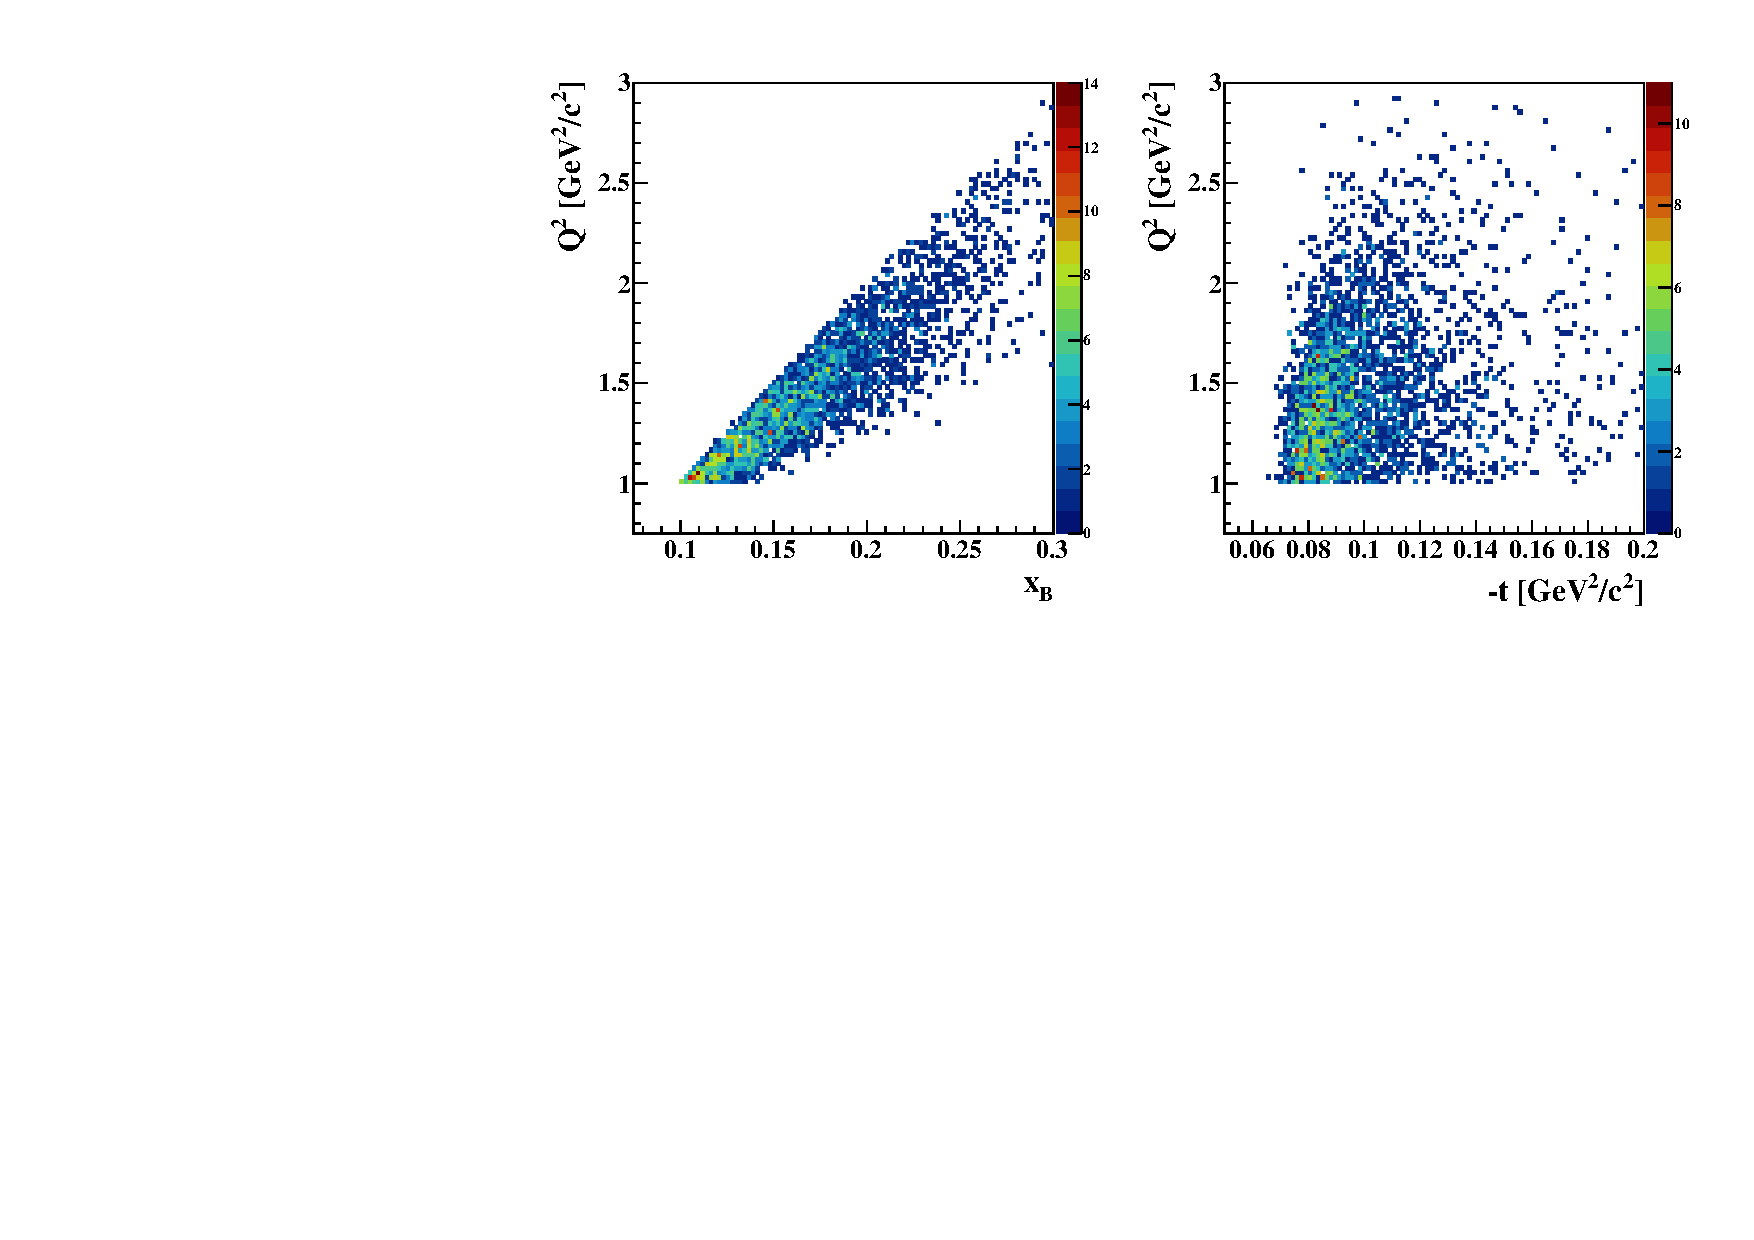
\includegraphics[width=9.0cm]{figs/Q2_xB_t_Coh.pdf}
\caption{Coherent DVCS event distributions for $Q^{2}$ as a function of 
$x_{B}$ (left) and $Q^{2}$ as a function of $-t$ (right) after the 
exclusivity cuts.}
\label{fig:kin-coverage}
\end{figure}

We identified two main backgrounds to our measurement, accidental 
coincidences and exclusive $\pi^0$ production. The accidental events have 
particles coming from different events, and we estimate their  contribution
to be 4.1\% of our sample. We evaluated this contribution by selecting events 
passing all our cuts but with an electron and an helium originating from different 
vertices. Regarding the $\pi^0$ production, it can easily be mistaken for DVCS when 
one of the two photons of the $\pi^0$ decay is produced at low energy in the 
laboratory frame and remains undetected. To estimate the importance of this 
background, we developed an event generator calibrated on the experimental yield 
of exclusive $\pi^0$ measured by our experiment. We used this generator together 
with a GEANT3 simulation of our detection system to estimate the ratio between
the number of $\pi^0$ events where the two photons are detected and those that 
would be mistaken for DVCS. This ratio is then multiplied by the measured yield 
of exclusive $\pi^0$ events to correct the DVCS data. Depending on the kinematics, we
found contaminations of 2 to 4\%. The study of systematics errors showed that the main 
contributions come from the choice of the DVCS exclusivity cuts (8\%) and the 
large binning size (5.1\%) [Is that right to add it here?]. However, added quadratically, these 
errors sum up to about 10\%, which always remain significantly smaller than the 
statistical errors.

%asymmetries
Several observables related to DVCS are of interest, but in this work we focus only 
on the beam-spin asymmetry. This  observable is measurable using a polarized 
lepton beam on an unpolarized target (U). It is convenient to use the beam-spin 
asymmetry because most of the experimental normalization and acceptance issues 
cancel out in the asymmetry ratio. It is defined in terms of the cross sections 
as:
  \begin{equation}
  A_{LU} = \frac{d^{5}\sigma^{+} - d^{5}\sigma^{-} }
                {d^{5}\sigma^{+} + d^{5}\sigma^{-}}.
    \label{BSA_equation}
  \end{equation}
where $d^{5}\sigma^{+(-)}$ is the DVCS differential cross 
section for a positive (negative) beam helicity. Experimentally, $A_{LU}$ 
can be expressed in terms of the measured number of events in each 
beam-helicity state ($N^{+}$, $N^{-}$) as:
\begin{equation}
A_{LU} = \frac{1}{P_{B}} \frac{N^{+} - N^{-}}{N^{+} + N^{-} }.
\end{equation}
where $P_{B}$ is the beam polarization, and $N^{+}$ and $N^{-}$ are the number 
of DVCS events detected with positive and negative electron helicity with 
respect to the beam direction. 

To interpret DVCS, one has to keep in mind that this reaction is 
indistinguishable from the Bethe-Heitler (BH) process, where the final photon 
is emitted either from the incoming or the outgoing leptons. At leading twist 
and leading order, the deeply virtual photon production cross section is 
composed of BH, DVCS, and interference terms. The amplitudes of the 
three terms can be approximated as a finite sum of Fourier harmonics, as shown 
for the nucleon in \cite{Belitsky:2001ns} and for the spin-zero targets in 
\cite{Kirchner:2003wt,Belitsky:2008bz}. Based on these calculations, the 
beam-spin asymmetry ($A_{LU}$) of a spin-zero hadron can then be expressed as:
\small
\begin{equation}
\begin{split}
A_{LU}(\phi) =~~~~~~~~~~~~~~~~~~~~~~~~~~~~~~~~~~~~~~~~~~~~~~~~~~~~~~~~~\\
 \frac{\alpha_{0}(\phi) \, \Im m(\mathcal{H}_{A})}
{\alpha_{1}(\phi) + \alpha_{2}(\phi) \, \Re e(\mathcal{H}_{A}) + \alpha_{3}(\phi) \, 
\big( 
\Re e(\mathcal{H}_{A})^{2} + \Im m(\mathcal{H}_{A})^{2} \big)}
\label{eq:A_LU-coh}
\end{split}
\end{equation}
\normalsize
where $\Im m(\mathcal{H}_{A})$ and $\Re e(\mathcal{H}_{A})$ are the imaginary 
and real parts of the $^4$He CFF $\mathcal{H}_{A}$ associated with the GPD $H_A$,
and $\phi$ is the azimuthal angle between the ($e$,$e'$) and 
($\gamma^{*}$,$^4$He$'$) planes. The $\alpha_{i}$'s are $\phi$-dependent 
kinematical factors that depend on the nuclear form factor ($F_{A}(t)$) and the 
independent variables $Q^2$, $x_{B}$ and $t$. These factors are expressed as:
\small
\begin{eqnarray}
   \alpha_0 (\phi) & = &\frac{x_{A}(1+\epsilon^2)^2}{y} S_{++}(1) \sin(\phi)\\
    \alpha_1 (\phi) & = & c_0^{BH}+c_1^{BH} \cos({\phi})+c_2^{BH} \cos(2\phi)\\ 
   \alpha_2 (\phi) & = & \frac{x_{A}(1+\epsilon^2)^2}{y}  \left( C_{++}(0) +  
C_{++}(1) cos(\phi) \right)\\
\alpha_3 (\phi) &=& \frac{x^{2}_{A}t(1+\epsilon^2)^2}{y} {\mathcal P}_1(\phi) 
{\mathcal P}_2(\phi) \cdot 2 \frac{2-2y+y^2 + \frac{\epsilon^2}{2}y^2}{1 + 
\epsilon^2}
\end{eqnarray}
\normalsize
Where $x_{A} = \frac{x_{B}M_{N}}{M_{A}}$ with $M_{A}$ the $^4$He mass and 
$\mathcal{P}_1(\phi)$ and $\mathcal {P}_2(\phi)$ the Bethe-Heitler
propagators. The factors $c_{0,1,2}^{BH}$, $c_0^{DVCS}$, $c_{0,1}^{INT}$ and
$s_1^{INT}$ are the Fourier coefficients of the BH, and $S{++}(1)$, $C_{++}(0)$, 
and $C_{++}(1)$ are the Fourier harmonics in the leptonic tensor. The 
explicit expressions of these terms can be found in \cite{Belitsky:2008bz}. 
We see that by using the $\sin(\phi)$ and $\cos(\phi)$ contributions, it is 
possible to extract 
$\Im m(\mathcal{H}_{A})$ and $\Re e(\mathcal{H}_{A})$ from the beam spin
asymmetry. 

Due to limited statistics, we only bin  our data two-dimensionally 
 in the azimuthal angle ($\phi$) and one of the kinemtical variables 
$Q^{2}$, $x_{B}$ and $t$. Figure \ref{fig:alu} presents $A_{LU}$ for the three
sets of binning. The asymmetries are fitted with the form of
equation \ref{eq:A_LU-coh}, where the real and imaginary part of the CFF
$\mathcal{H}_{A}$ are the free parameters of the fit. Figure \ref{fig:alu90} 
shows the $Q^2$, $x_{B}$, and $-t$-dependencies of the fitted $A_{LU}$ signals 
at $\phi$~=~90$^{\circ}$. The $x_{B}$ and $-t$-dependencies are compared to 
theoretical calculations performed by S.~Liuti and K.~Taneja 
\cite{simonetta_2}. Their model relies on the impulse approximation and uses 
advanced spectral functions of nuclei. The calculations are at slightly different 
kinematics than our data but still provide some guidance. The experimental 
results appear to have larger asymmetries than the calculations. These 
differences may arise from nuclear effects which are not taken into account in 
the model, such as long-range interactions.

\begin{figure}[tb]
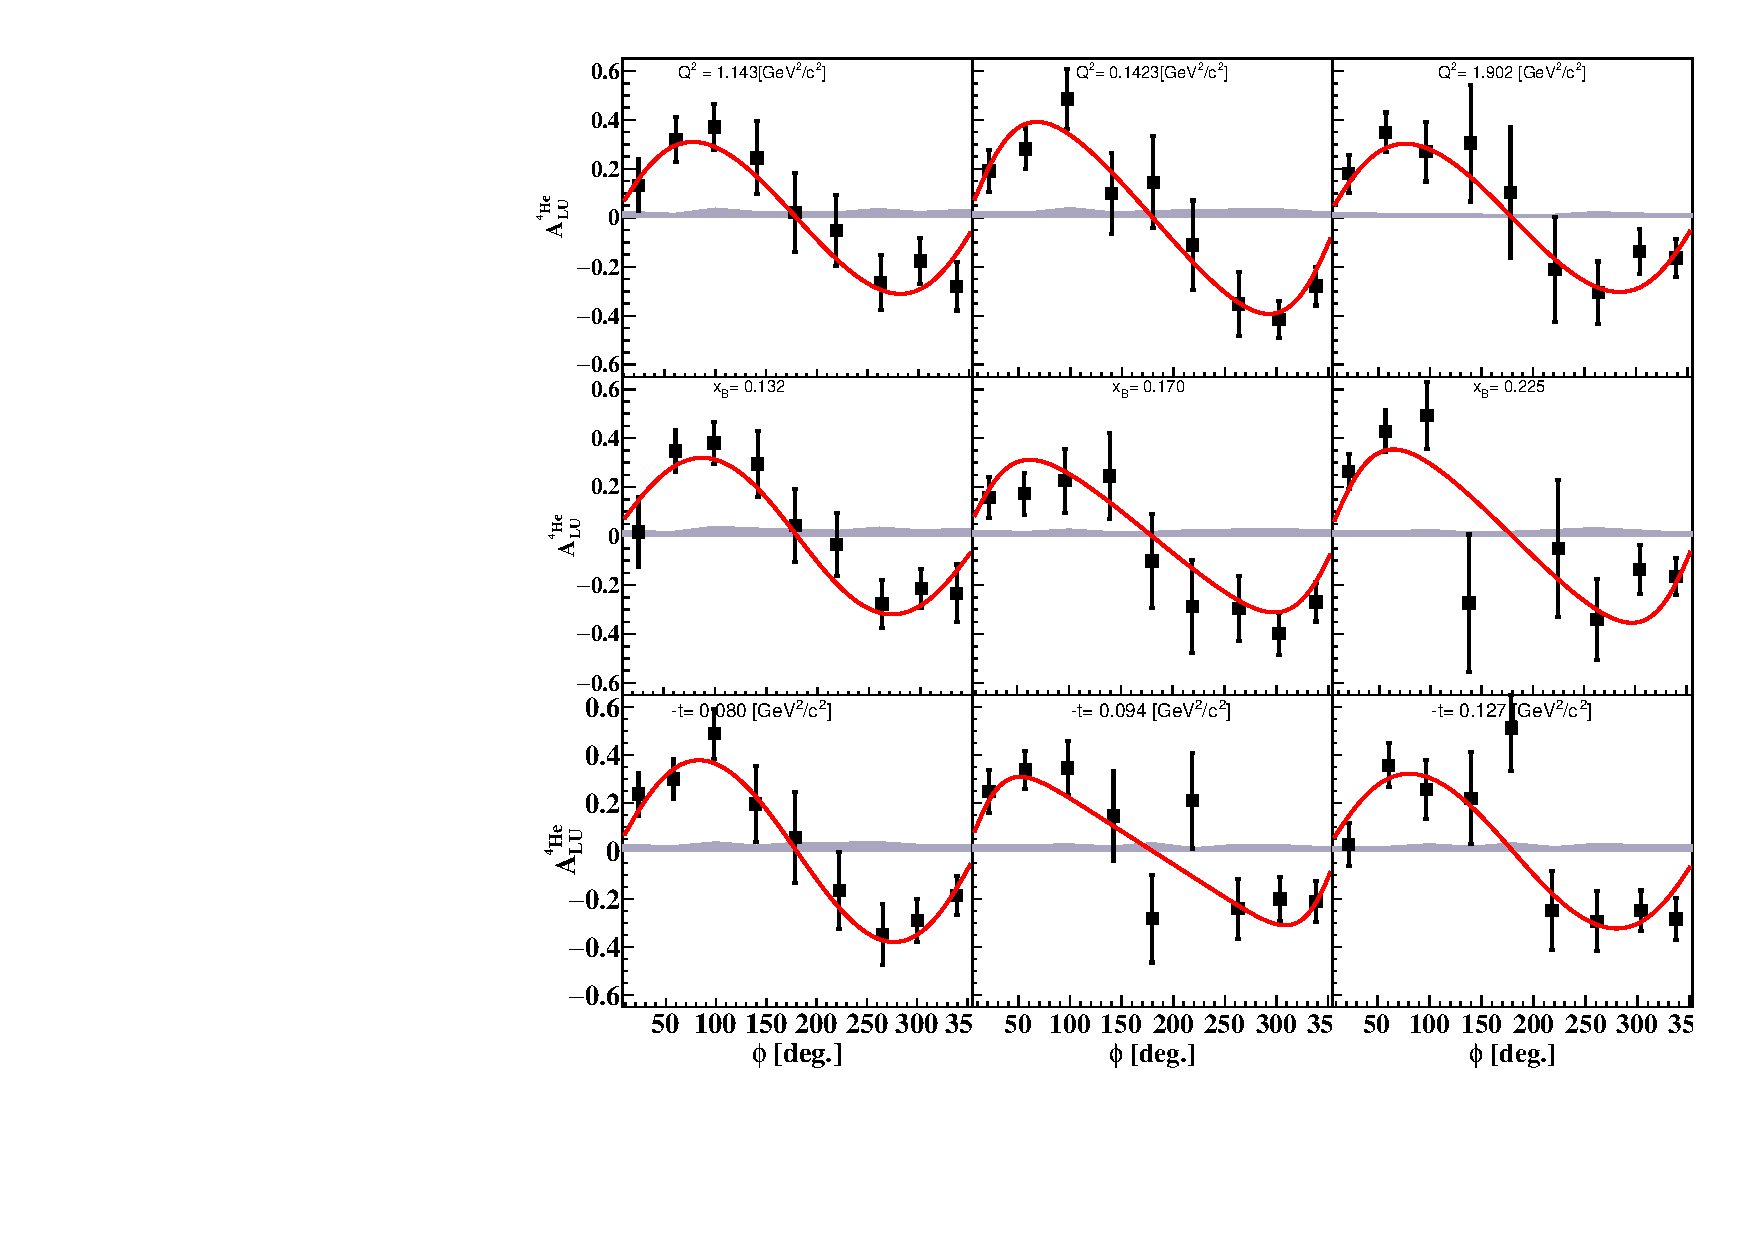
\includegraphics[width=8.9cm]{figs/coherent-ALU.pdf}
\caption{The coherent $A_{LU}$ as a function of $\phi$. Results are presented
   for different $Q^{2}$ bins (top panel), $x_{B}$ bins (middle panel), and 
   $-t$ bins (bottom panel).  
   The error bars represent the statistical uncertainties. The gray 
   bands represent the systematic uncertainties, including the normalisation 
   uncertainties. The red curves are the results of our fits with the form of 
   equation \ref{eq:A_LU-coh}.}
\label{fig:alu}
\end{figure}

\begin{figure}[tb]
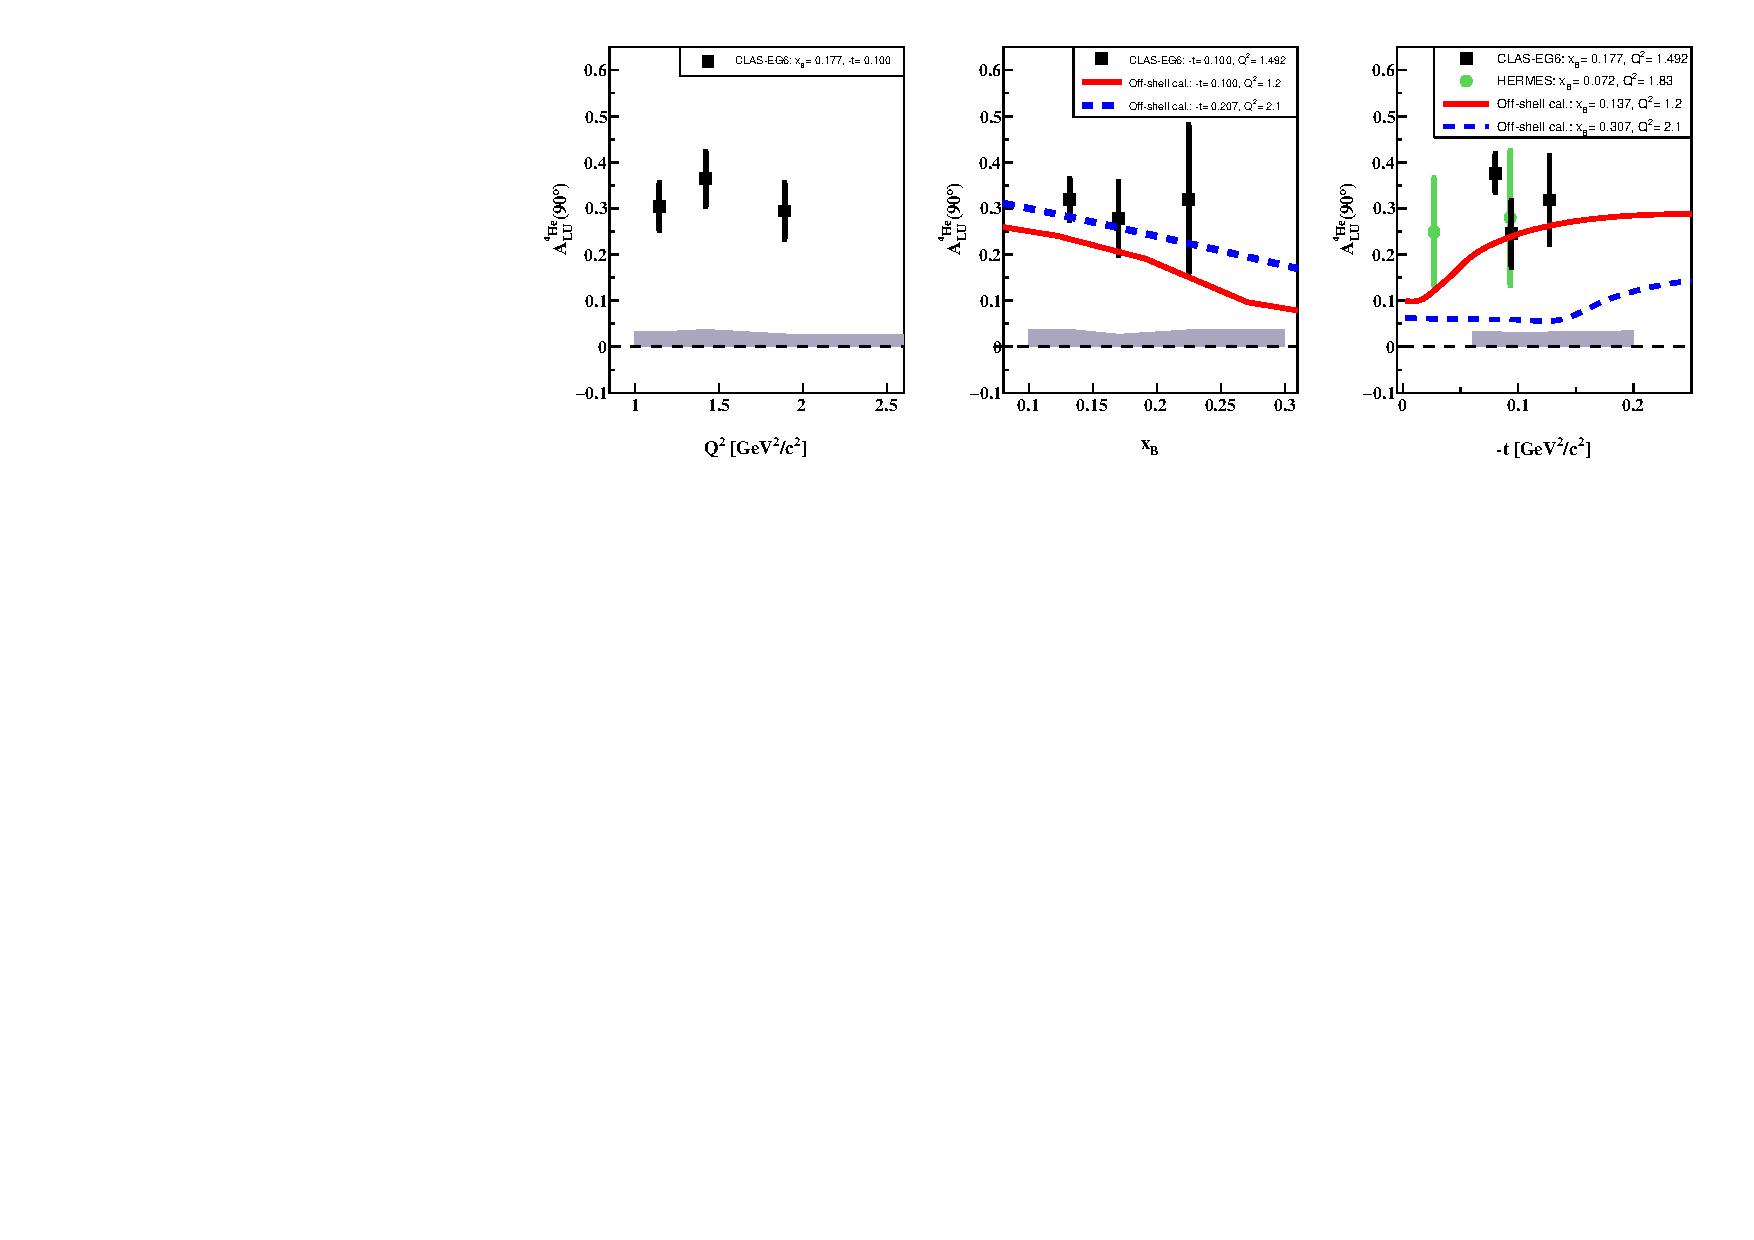
\includegraphics[width=8.9cm]{figs/coherent-ALU_90.pdf}
\caption{The $Q^{2}$ (left), $x_{B}$ (middle), and $-t$-dependencies (right) of
   the $A_{LU}$ at $\phi$~=~90$^{\circ}$ (black squares). On the 
   middle plot: the full-red and the dashed-blue curves are theoretical 
   calculations from \cite{simonetta_2}. On the right: the green circles are 
   the HERMES $-A_{LU}$ (positron beam was used) inclusive measurements 
   \cite{HERMES_BSA}, the colored curves represent theoretical calculations 
   from \cite{simonetta_2}.}
\label{fig:alu90}
\end{figure}


\begin{figure}[tb]
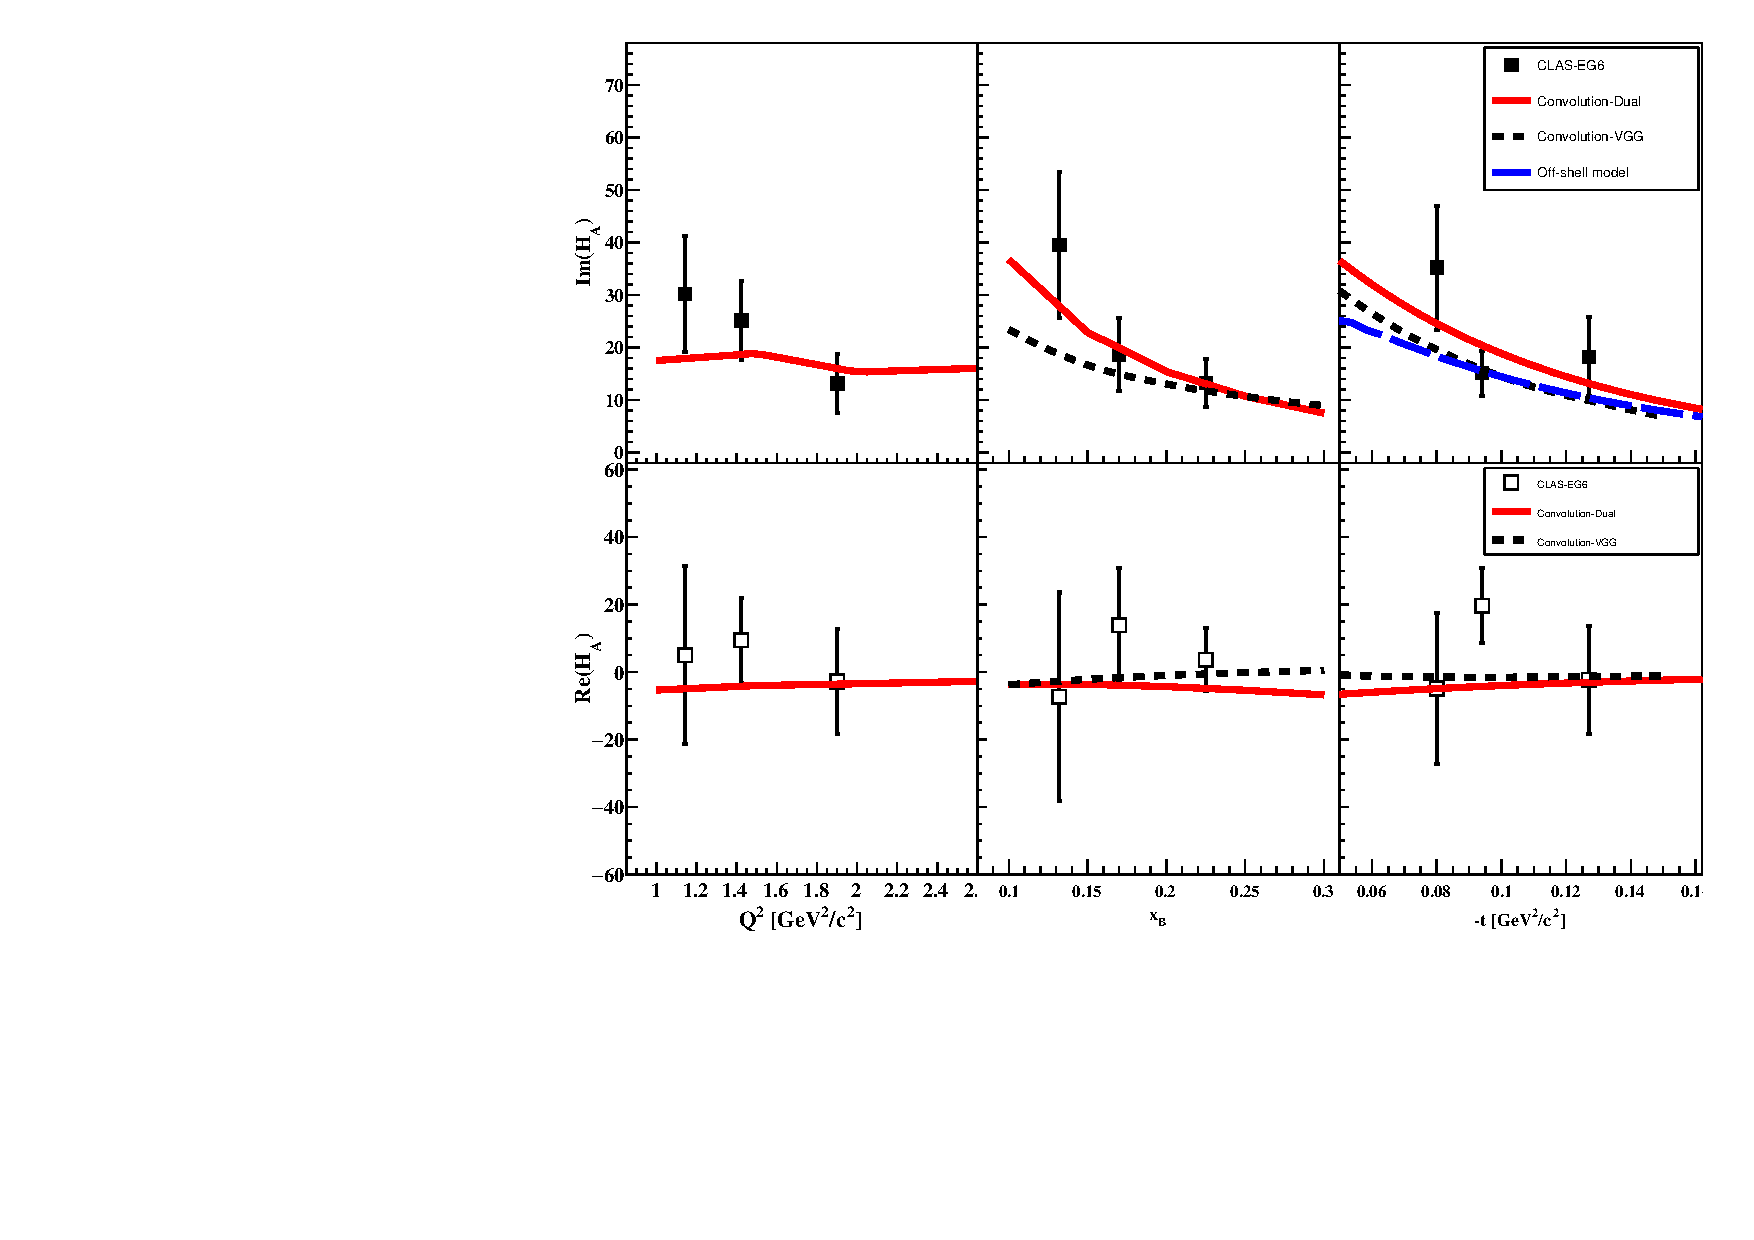
\includegraphics[width=8.9cm]{figs/Coherent_CFF.pdf}
\caption{The model-independent extraction of the imaginary (top panel) and
real (bottom panel) parts of the $^4$He CFF $\mathcal{H}_A$, as functions of
$Q^{2}$ (right panel), $x_B$ (middle panel), and $t$ (left panel). The full red 
curves are calculations based on an on-shell model from
\cite{Vadim_priv}. The black-dashed curves are calculations from a convolution 
model based on the VGG model for the nucleons' GPDs \cite{Guidal_priv}. The 
blue long-dashed curve on the top-right plot is from
an off-shell model based on \cite{GonzalezHernandez:2012jv}.}
\label{fig:CFF_HA}
\end{figure}

We display in figure \ref{fig:CFF_HA} our extraction of the $^4$He CFF 
$\mathcal{H}_A$, together with theoretical calculations from two models, 
labelled {\em convolution} and {\em off-shell}. In the convolution 
model \cite{Vadim_priv}, the nucleus is assumed to be composed of 
non-relativistic non-interacting nucleons, where these nucleons interact 
independently with the probe. The convolution/dual model is based on nucleon GPDs from 
the dual parametrization \cite{Guzey:2006xi}, where the convolution/VGG uses nucleon GPDs  
from the VGG model and is based on the double distributions ansatz 
\cite{DD_model}. The off-shell model \cite{GonzalezHernandez:2012jv} relies on the 
impulse approximation and uses advanced spectral functions of  
nuclei that account for all configurations of the final nuclear system and the 
binding effects between the nucleons.
[These need to be renamed on the figure, it does not make sense to call differently
models that are identical. We should also request the projections from Vadim
model: hep-ph/0509158.]

The results in Figure \ref{fig:CFF_HA} show that the extraction of the CFF
from the beam spin asymmetry is possible without any model dependent 
assumptions. The amplitude and the dependencies observed as a function of 
$Q^{2}$, $x_B$, and $-t$ are in agreement 
with the theoretical calculations. One can see a difference between the 
precision of the extracted imaginary and real parts, which is expected from
equation \ref{eq:A_LU-coh} because $\alpha_2$ is smaller than $\alpha_0$. 
While these results are not precise enough to discriminate between the models,
they are very promising for future exeperiments and demonstrate our ability
to directly extract the CFF of the helium nucleus in a completely model
independent way.


%conclusion
In summary, we present the first exclusive measurement of coherent DVCS 
off $^4$He using the CLAS spectrometer supplemented  
by a specially designed RTPC. This dataset represents a 
unique source as the first exclusive coherent nuclear DVCS measurement which 
can be used to directly constrain GPD models. The measured beam-spin asymmetries 
show a signal stronger than for the proton and allow to perform a fully 
model-independent extraction of the $^4$He CFF $\mathcal{H}_A$. The extracted 
CFF is in a good agreement with the available models. This opens 
many new perspectives to study the nuclear structure within the GPD framework 
and paves the way for future, more precise measurements at JLab 12~GeV to 
eventualy localize nuclear effects in the transverse plane.


%Acknowledgments

We acknowledge the staff of the Accelerator and Physics Divisions at Jefferson 
Lab for making this experiment possible. This work is supported by the U.S.  
Department of Energy, Office of Science, Office of Nuclear Physics contract 
DE-AC05-06OR23177.

\begin{thebibliography}{99}
\bibitem{Mueller:1998fv} 
D. Mueller, D. Robaschik, B. Geyer, F.M. Dittes and J. Horejsi,
Fortsch.\ Phys. {\bf 42}, 101 (1994).
  
\bibitem{Ji:1996ek} 
X.D. Ji,
Phys.\ Rev.\ Lett. {\bf 78}, 610 (1997).

\bibitem{Ji:1996nm} 
X.D. Ji,
Phys.\ Rev.\ D {\bf 55}, 7114 (1997).

\bibitem{Radyushkin:1996nd}
A.V. Radyushkin,
Phys.\ Lett.\  B {\bf 380}, 417 (1996).

\bibitem{Radyushkin:1997ki} 
A.V. Radyushkin,
Phys.\ Rev.\ D {\bf 56}, 5524 (1997).

\bibitem{Burkardt:2000za} 
  M.~Burkardt,
  Phys.\ Rev.\ D {\bf 62}, 071503 (2000)
  Erratum: Phys.\ Rev.\ D {\bf 66}, 119903 (2002)

\bibitem{Diehl:2002he} 
  M.~Diehl,
  Eur.\ Phys.\ J.\ C {\bf 25}, 223 (2002)
  Erratum: Eur.\ Phys.\ J.\ C {\bf 31}, 277 (2003)
 
\bibitem{Belitsky:2002ep} 
  A.~V.~Belitsky and D.~Mueller,
  Nucl.\ Phys.\ A {\bf 711}, 118 (2002)

\bibitem{Burkardt:2005hp} 
  M.~Burkardt,
  Phys.\ Rev.\ D {\bf 72}, 094020 (2005)

\bibitem{Stepanyan:2001sm}
S.~Stepanyan {\it et al.} [CLAS Collaboration],
Phys.\ Rev.\ Lett. {\bf 87}, 182002 (2001).

\bibitem{Airapetian}
A. Airapetian {\it et al.} [HERMES Collaboration],
Phys.\ Rev.\ Lett. {\bf 87}, 182001 (2001);
JHEP {\bf 1207}, 032 (2012);
JHEP {\bf 1006}, 019 (2010);
JHEP {\bf 0806}, 066 (2008);
Phys.\ Lett.\ B {\bf 704}, 15 (2011);
Phys.\ Rev.\  D {\bf 75}, 011103 (2007);
JHEP {\bf 0911}, 083 (2009);
Phys.\ Rev.\ C {\bf 81}, 035202 (2010);
JHEP {\bf 1210}, 042 (2012).

\bibitem{Chekanov:2003ya}
S. Chekanov {\it et al.} [ZEUS Collaboration],
Phys.\ Lett.\  B {\bf 573}, 46 (2003).

\bibitem{Aktas:2005ty}
A. Aktas {\it et al.} [H1 Collaboration],
Eur.\ Phys.\ J.\ C {\bf 44}, 1 (2005).

\bibitem{Chen:2006na} 
S.~Chen {\it et al.} [CLAS Collaboration],
Phys.\ Rev.\ Lett.\ {\bf 97}, 072002 (2006).

\bibitem{Munoz Camacho:2006hx} 
C. Mu\~noz Camacho {\it et al.} [Jefferson Lab Hall A Collaboration],
Phys.\ Rev.\ Lett. {\bf 97}, 262002 (2006).

\bibitem{Girod:2007aa} 
F.X. Girod {\it et al.} [CLAS Collaboration],
Phys.\ Rev.\ Lett. {\bf 100}, 162002 (2008).

\bibitem{Mazouz:2007aa} 
   M.~Mazouz {\it et al.} [Jefferson Lab Hall A Collaboration],
   Phys.\ Rev.\ Lett.\  {\bf 99}, 242501 (2007)

\bibitem{Gavalian:2009} 
G. Gavalian {\it et al.} [CLAS Collaboration],
Phys.\ Rev.\ C {\bf 80}, 035206 (2009).

\bibitem{Seder:2015} 
E. Seder {\it et al.} [CLAS Collaboration],
Phys.\ Rev.\ Lett. {\bf 114}, 032001 (2015).

\bibitem{Pisano:2015} 
S.~Pisano {\it et al.} [CLAS Collaboration],
Phys.\ Rev.\ D {\bf 91}, 052014 (2015).

\bibitem{Jo:2015ema} H.~S.~Jo {\it et al.} [CLAS Collaboration],
  Phys.\ Rev.\ Lett.\  {\bf 115}, no. 21, 212003 (2015)

\bibitem{Goeke:2001tz}
K. Goeke, M.V. Polyakov and M. Vanderhaeghen,
Prog.\ Part.\ Nucl.\ Phys. {\bf 47}, 401 (2001).

\bibitem{Diehl:2003ny}
M. Diehl,
Phys.\ Rept.  {\bf 388}, 41 (2003).

\bibitem{Ji:2004gf}
X.D. Ji,
Ann.\ Rev.\ Nucl.\ Part.\ Sci. {\bf 54}, 413 (2004).

\bibitem{Belitsky:2005qn}
A.V. Belitsky and A.V. Radyushkin,
Phys.\ Rept. {\bf 418}, 1 (2005).

\bibitem{Boffi:2007yc} S. Boffi and B. Pasquini,
Riv.\ Nuovo Cim. {\bf 30}, 387 (2007).

\bibitem{Guidal:2013rya} 
M.~Guidal, H.~Moutarde and M.~Vanderhaeghen,
Rept.\ Prog.\ Phys.\  {\bf 76}, 066202 (2013).

\bibitem{Dupre:2015jha} 
  R.~Dupr\'e and S.~Scopetta,
  Eur.\ Phys.\ J.\ A {\bf 52}, no. 6, 159 (2016)

\bibitem{Hen:2016kwk} 
  O.~Hen, G.~A.~Miller, E.~Piasetzky and L.~B.~Weinstein,
  arXiv:1611.09748 [nucl-ex].

\bibitem{Norton:2003cb} 
  P.~R.~Norton,
  Rept.\ Prog.\ Phys.\  {\bf 66}, 1253 (2003).

\bibitem{Geesaman:1995yd} 
  D.~F.~Geesaman, K.~Saito and A.~W.~Thomas,
  Ann.\ Rev.\ Nucl.\ Part.\ Sci.\  {\bf 45}, 337 (1995).

\bibitem{Freund_Collins}
A.~Freund and J.C.~Collins, 
Phys.\ Rev.\ D {\bf 59}, 074009 (1998)

\bibitem{Ji_Osborne}
X.-D.~Ji and J.~Osborne, 
Phys.\ Rev.\ D {\bf 58}, 094018 (1998)

\bibitem{Ellinghaus:2002zw}
F.~Ellinghaus {\it et al.} [HERMES Collaboration],
AIP Conf.\ Proc.\  {\bf 675}, 303 (2003)

\bibitem{Guzey:2003jh} 
  V.~Guzey and M.~Strikman,
  Phys.\ Rev.\ C {\bf 68}, 015204 (2003)

\bibitem{JSeely}
J. Seely {\it et al.} 
Phys.\ Rev.\ Lett.\ {\bf 103}, 202301 (2009)

\bibitem{Mecking:2003zu} 
   B.~A.~Mecking {\it et al.} [CLAS Collaboration],
   Nucl.\ Instrum.\ Meth.\ A {\bf 503}, 513 (2003).

\bibitem{Belitsky:2001ns}
A.~V.~Belitsky, D.~Mueller and A.~Kirchner,
Nucl.\ Phys.\ B {\bf 629}, 323 (2002)

\bibitem{Kirchner:2003wt}
A.~Kirchner and D.~Mueller, 
Eur.\ Phys.\ J.\ C {\bf 32}, 347 (2003)

\bibitem{Belitsky:2008bz}
A.~V.~Belitsky and D.~Mueller,
Phys.\ Rev.\ D {\bf 79}, 014017 (2009)

%\bibitem{eg6_note}
%M. Hattawy {\it et al.} (CLAS-EG6 Working Group), CLAS internal analysis note, 
%2016.

\bibitem{simonetta_2}
S.~Liuti and K.~Taneja, 
Phys.\ Rev.\ C {\bf 72}, 032201 (2005)

\bibitem{Vadim_priv}
Private communications with V.~Guzey based on: 
V.~Guzey, Phys.\ Rev.\ C {\bf 78}, 025211 (2008).

\bibitem{Guzey:2006xi}
V.~Guzey and T.~Teckentrup,
Phys.\ Rev.\ D {\bf 74}, 054027 (2006)

\bibitem{Guidal_priv}
Private communications with M.~Guidal based on: 
M.~Guidal, M.~V.~Polyakov, A.~V.~Radyushkin and M.~Vanderhaeghen, 
Phys.\ Rev.\ D {\bf 72}, 054013 (2005).

\bibitem{DD_model}
I.~V.~Musatov and A.~V.~Radyushkin, 
Phys.\ Rev.\ D {\bf 61}, 074027 (2000).

\bibitem{GonzalezHernandez:2012jv}
Private communications with S.~Liuti based on: 
J.~O.~Gonzalez-Hernandez, S.~Liuti, G.~R.~Goldstein and K.~Kathuria,
Phys.\ Rev.\ C {\bf 88}, no. 6, 065206, (2013).


\end{thebibliography}

\end{document}
